% -----------------------------------------------------------------------------
% Implementation
% -----------------------------------------------------------------------------
\chapter{Implementation}
\label{chap:implementation}
\section{Image Source Method}
The implementation of the image source model will unfold in several steps. Building up from a rudimentary to a more complex and realistic implementation.
\subsection{Images Source Model with 4 walls - image order 1}
We start by modeling a simple room with only 4 walls (no ceiling or floor) with a receiver positioned at the point (single source positioned at the point $P(1,1,1)$ and its reflection of the first order relative to the walls as seen in figure \ref{fig:ism_4_1}\\
\begin{figure}
    \centering
    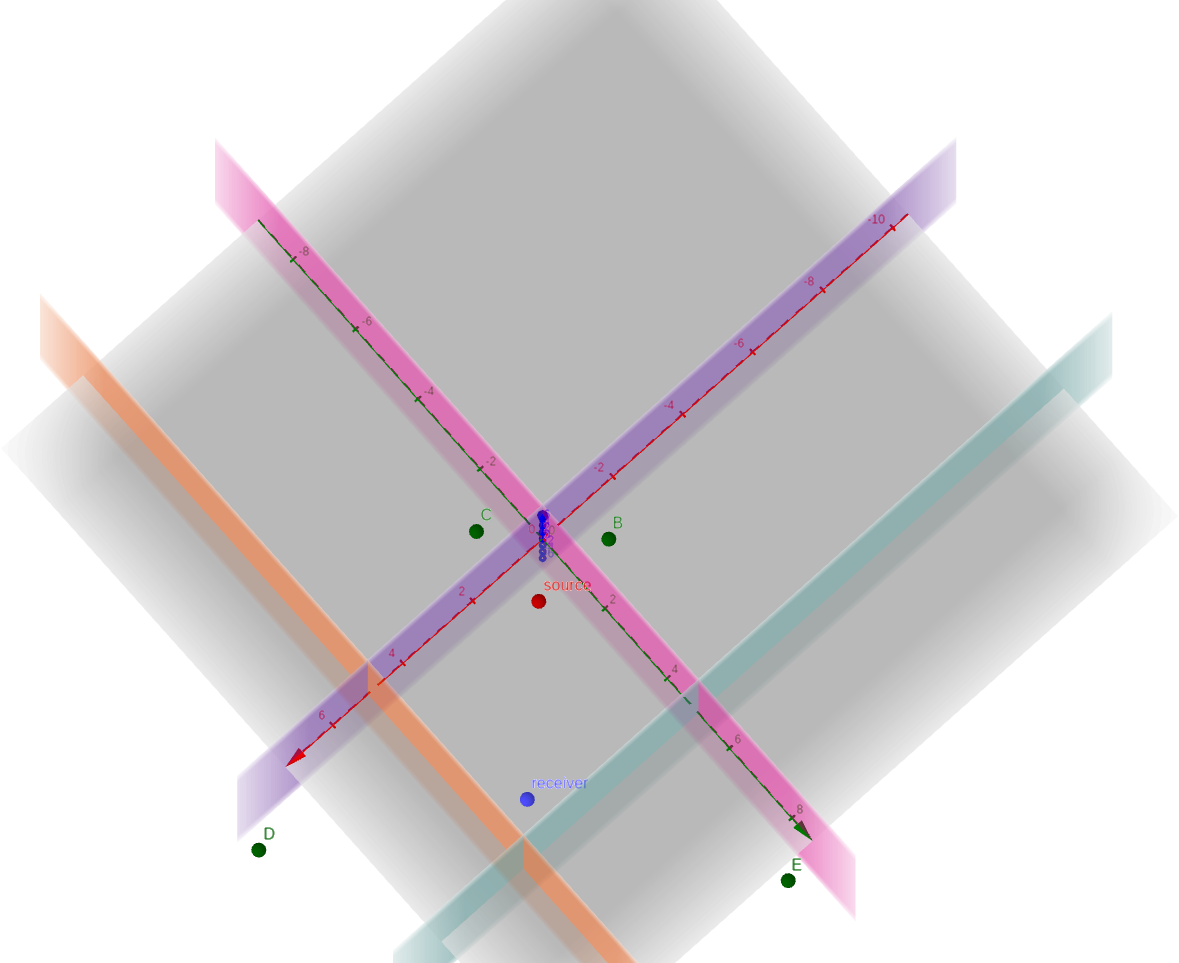
\includegraphics[width=1\textwidth,keepaspectratio]{LaTeX/images/geometrie/ism_4_walls_order_1.png}\\
    \caption{Source and receiver in room with 4 walls and reflections of order 1}
    \label{fig:ism_4_1}
\end{figure}
